% -----------------------------------------------
% Template for SMAC SMC 2013
% adapted and corrected from the template for SMC 2012, which was adapted from that of SMC 2011
% further updated for TENOR 2015, 2016, 2017 and 2020
% -----------------------------------------------

\documentclass{article}
\usepackage{tenor2021}
\usepackage{ifpdf}
\usepackage[english]{babel}
\usepackage{balance}
\usepackage{color}
\usepackage{float}
%\usepackage{rail}

%%%%%%%%%%%%%%%%%%%%%%%% Some useful packages %%%%%%%%%%%%%%%%%%%%%%%%%%%%%%%
%%%%%%%%%%%%%%%%%%%%%%%% See related documentation %%%%%%%%%%%%%%%%%%%%%%%%%%
%\usepackage{amsmath} % popular packages from Am. Math. Soc. Please use the 
%\usepackage{amssymb} % related math environments (split, subequation, cases,
%\usepackage{amsfonts}% multline, etc.)
%\usepackage{bm}      % Bold Math package, defines the command \bf{}
%\usepackage{paralist}% extended list environments
%%subfig.sty is the modern replacement for subfigure.sty. However, subfig.sty 
%%requires and automatically loads caption.sty which overrides class handling 
%%of captions. To prevent this problem, preload caption.sty with caption=false 
%\usepackage[caption=false]{caption}
%\usepackage[font=footnotesize]{subfig}


%user defined variables
\def\papertitle{A Web Based Environment Embedding Signal Processing in Music Scores}
\def\allauthors{Dominique Fober \hskip .2in Yann Orlarey \hskip .2in Stéphane Letz \hskip .2in Romain Michon}
\def\firstauthor{Dominique Fober}
\def\secondauthor{Yann Orlarey}
\def\thirdauthor{Stéphane Letz}
\def\fourthauthor{Romain Michon}

% adds the automatic
% Saves a lot of ouptut space in PDF... after conversion with the distiller
% Delete if you cannot get PS fonts working on your system.

% pdf-tex settings: detect automatically if run by latex or pdflatex
\newif\ifpdf
\ifx\pdfoutput\relax
\else
   \ifcase\pdfoutput
      \pdffalse	
   \else
      \pdftrue
\fi

\ifpdf % compiling with pdflatex
  \usepackage[pdftex,
    pdftitle={\papertitle},
    pdfauthor={\firstauthor, \secondauthor, \thirdauthor},
    bookmarksnumbered, % use section numbers with bookmarks
    pdfstartview=XYZ % start with zoom=100% instead of full screen; 
                     % especially useful if working with a big screen :-)
   ]{hyperref}
  %\pdfcompresslevel=9

  \usepackage[pdftex]{graphicx}
  % declare the path(s) where your graphic files are and their extensions so 
  %you won't have to specify these with every instance of \includegraphics
  \graphicspath{{./figures/}}
  \DeclareGraphicsExtensions{.pdf,.jpeg,.png}

  \usepackage[figure,table]{hypcap}

\else % compiling with latex
  \usepackage[dvips,
    bookmarksnumbered, % use section numbers with bookmarks
    pdfstartview=XYZ % start with zoom=100% instead of full screen
  ]{hyperref}  % hyperrefs are active in the pdf file after conversion

  \usepackage[dvips]{epsfig,graphicx}
  % declare the path(s) where your graphic files are and their extensions so 
  %you won't have to specify these with every instance of \includegraphics
  \graphicspath{{./figures/}}
  \DeclareGraphicsExtensions{.eps}

  \usepackage[figure,table]{hypcap}
\fi

%setup the hyperref package - make the links black without a surrounding frame
\hypersetup{
    colorlinks=true,%
    citecolor=black,%
    filecolor=black,%
    linkcolor=mylink,%
    urlcolor=black
}


% Title.
% ------
\title{\papertitle}

% Authors
% Please note that submissions are NOT anonymous, therefore 
% authors' names have to be VISIBLE in your manuscript. 
%
% Single address
% To use with only one author or several with the same address
% ---------------
\oneauthor
   {\allauthors} {Grame-CNCM \\ %
     {\tt \href{mailto:fober@grame}{fober@grame.fr}}}

%Two addresses
%--------------
% \twoauthors
%   {\firstauthor} {Affiliation1 \\ %
%     {\tt \href{mailto:author1@adomain.org}{author1@adomain.org}}}
%   {\secondauthor} {Affiliation2 \\ %
%     {\tt \href{mailto:author2@adomain.org}{author2@adomain.org}}}

% Three addresses
% --------------
% \fourauthors
%   {\firstauthor} {Grame-CNCM \\ %
%     {\tt \href{mailto:fober@grame.fr}{fober@grame.fr}}}
%   {\secondauthor} {Grame-CNCM \\ %
%     {\tt \href{mailto:orlarey@grame.fr}{orlarey@grame.fr}}}
%   {\thirdauthor} {Grame-CNCM \\ %
%     {\tt \href{mailto:letz@grame.fr}{letz@grame.fr}}}
%   {\fourthauthor} { Grame-CNCM \\ %
%     {\tt \href{mailto:michon@grame.fr}{michon@grame.fr}}}

% user commands

\definecolor{mygrey}{gray}{0.95}
\definecolor{mylink}{rgb}{0.384,0.0,0.145}

\newcommand{\ispace}	{\setlength\itemsep{0mm}}
\newcommand{\icode}[1]	{{\small \texttt{#1}}}
\newcommand{\code}[1]	{\vspace{-1em}\begin{center}\colorbox{mygrey}{\begin{minipage}[t]{0.98\columnwidth} {\scriptsize \texttt{#1}}\end{minipage}}\end{center}}

\newcommand{\osctype}[1]	{\textbf{\texttt{{\small #1}}}}
\newcommand{\oscint}		{\osctype{int32}}
\newcommand{\oscfloat}		{\osctype{float32}}
\newcommand{\oscstring}		{\osctype{string}}

%\railparam{\addtolength{\itemsep}{-3ex}}
%\setlength\railnamesep{-1mm}
%\railterm{int32, float32, string}
%\railalias{int32}{\oscint}
%\railalias{float32}{\oscfloat}
%\railalias{string}{\oscstring}

% ***************************************** the document starts here ***************
\begin{document}
%
\capstartfalse
\maketitle
\capstarttrue
%
%=========================================================
\begin{abstract}
We present an online environment for the design of musical scores, which also allows the embedding of signal processors and thus the publication of electronic works. This environment is part of the INScore project, which latest version has been transcribed into WebAssembly/Javascript, to provide in a web browser both the diversity of music representations supported by INScore, the interaction capabilities and all the dynamic aspects of the score as offered by the native version.

After some historical elements about distributed music scores, we will make some reminders about the INScore project and its associated description language. We will then describe the architecture of the system and the choices made for its portability to the Web. Then we will present the extensions specific to the Javascript version and in particular the support of signal processing objects. 
Finally, we will show how INScore's communication system has been extended to allow online partition control from a native version of INScore, paving the way for real-time performance on the web.

\end{abstract}


%=========================================================
\section{Introduction}\label{sec:introduction}

Music notation tools have been investigating their deployment on the Internet since the late 1990s. The Guido Note Server \cite{renz98}, designed as a client-server architecture and based on the Guido Music Description Language \cite{hoos98} GMN] is an example of such a system. It will be followed by a large number of applications offering online music editing services, in a design modeled on traditional score editors (e.g. such as MuseScore\footnote{MuseScore \url{https://musescore.com/}}), enhanced by sharing services. 
In this area, we can mention Noteflight\footnote{Noteflight \url{https://www.noteflight.com/}}, Scorio\footnote{Scorio \url{https://www.scorio. com/}} or also, in the line of description languages associated to compilers, LilyBin\footnote{LilyBin \url{http://lilybin.com/}} or the GuidoEditor\footnote{GuidoEditor \url{https://guidoeditor.grame.fr/}}, the latter having the particularity to embed the compiler in a web page.
All these systems are turned to a traditional approach of musical notation and do not deal with problems related to network performances.

It is more recently and often thanks to the impulse of composers, that distributed score systems have emerged.
Quintet.net \cite{doi:10.1162/leon.2005.38.1.23}, an interactive Internet performance environment enabling up to five performers to play music in real-time over the Internet under the control of a \emph{conductor}, is among the first performance-oriented notation systems. 
The Decibel Score Player \cite{Hope_tenor2015} is another approach to distributed music score, based on a purely graphic notation of the music (as opposed to symbolic notation). It allows to synchronize the scores of a performing ensemble.
However, these systems are implemented as native applications (Quintet.net is based on Max/MSP and the Decibel Score Player is a standalone application for iPad) and therefore may be difficult to distributed on the web.

Facing similar problems, SmartVox \cite{bell:hal-01660184} uses a standard browser to distribute and synchronize music scores, which are also accompanied by audio signals. In the same line but with a focus on improvised music, John, the semi-conductor\cite{goudard:hal-01923258} is another web-based approach of music notation.
It is more recently that Drawsocket \cite{Gottfried_tenor2019} appears, a platform for generating synchronized, browser-based scores across an array of networked devices. Firmly rooted in web technologies (SVG, CSS, HTML and Javascript), it provides an API to develop networked scores.

Naturally turned to network communication, INScore \cite{Fober:12a} (presented in section \ref{sec:inscore}) is also open to web uses \cite{Fober:15b}, in particular due to web server objects (\icode{http} or \icode{websocket}) that can be embedded in a score, and by providing a basic Web API allowing to interact with the score from a browser. 
However, this approach is based on the native application and constrains its use to a client/server architecture, which limits both the ability to interact with the score as well as its dynamic aspects. 
We have therefore developed a Javascript version of the INScore environment, in the form of a library to be integrated into a web page as a stand-alone engine. 
Taking advantage of the modular architecture of the Web, in particular thanks to the Node Package Manager (NPM), this implementation makes it possible to embed the Faust compiler \cite{orlarey:hal-02159014} \cite{ren:hal-03087763} and thus to provide signal processing objects within the score.
A simple extension of the existing communication scheme can also be used to control a web score from the native version of INScore.

The next section is a quick reminder of INScore's approach to music representation. The following sections will detail the more technical aspects of the implementation for the web, the integration of Faust objects and the extension of the communication scheme, before concluding with the new perspectives offered by this environment and future work.


%=========================================================
\section{INScore Environment}\label{sec:inscore}

INScore is an environment for the design of augmented, dynamic and interactive music scores \cite{Fober:12a}, result of numerous research works that deal in particular with the extension of music notation to arbitrary graphic objects, time synchronisation in the graphic space \cite{fober:10b}, dynamic and interactive scores \cite{Fober:13b}, performance representation \cite{fober12tr} and the extension of the score to network dimensions \cite{Fober:15b}.
The design of a score is based on a specific scripting language and therefore also addresses the field of programming languages for the description of music \cite{fober:hal-02368958}. 

\subsection{Extended scores}
INScore allows you to extend the symbolic notation, or even replace it, with arbitrary graphic objects: images, text, vectorial drawing, video. All these objects, including symbolic notation, have the same status as musical objects and have an identical temporal dimension (i.e. date, duration and tempo). This lack of hierarchy allows these objects to be synchronised in arbitrary combinations.

\subsection{Representing the time of heterogeneous objects}
INScore takes advantage of the homogenous temporal dimension of the score objects to provide what we call \emph{time synchronisation in the graphic space}, which makes it possible to represent the temporal relationships between objects using a synchronisation mechanism. If we imagine that each pixel of an object carries a date (computed from the date and duration of the object) the synchronisation system potentially makes it possible to graphically align all the pixels of two or more objects, carrying the same date. The design of a cursor positioned at the current date of a score is achieved with a simple synchronisation command. But above all, it becomes possible to reason in temporal space and therefore in a metaphor close to musical thought, the rendering engine automatically \emph{translate} the temporal dimensions in the graphic space.

\subsection{Dynamic and interactive scores}

The notion of \emph{tempo} is an integral part of the temporal dimension of objects. By default, this tempo is set to zero: the object is motionless in time. When the tempo value is not zero, the object then moves in time at the speed specified by its tempo. Associated with the synchronisation system, the use of the tempo allows you to create dynamic scores, whose form and content can evolve autonomously in time.

An interaction system complements these dynamic aspects. The time of a score, conceived as musical time, relative to a tempo, can also be \emph{event based}, i.e. relative to asynchronuous events, which can be programmed in an arbitrary way. Among these events are the classic user interfaces events (such as mouse clicks, for example) but also \emph{temporal} events, whose occurrence depends on the flow of time. Each object in the partition is therefore capable of monitoring arbitrary events, including in the time domain: each event is associated with a set of messages that will be triggered at each occurrence of the event. These messages, expressed in INScore's scripting language, potentially allow the re-programming of all or part of the partition.

\subsection{The network dimensions of the music score}

INScore was originally designed to be driven by Open Sound Control [OSC] messages. It is therefore particularly suited to networks and the exchange of messages between INScore scores are native features. A simple \emph{message forwarding} system, allows a score to control a set of other scores distributed over a local area network, or to build a distributed music system on a client/server model \cite{Zagorac_tenor2018}.

As mentioned before, a score can also embed a web server, making it available from the Internet and providing control from a browser. On the other hand, the objects of a score can refer to resources distributed over the Internet, similarly to a browser that can aggregate content from different websites.

\subsection{INScore scripting language}
A score is described in a specific scripting language, which consists of a textual form of OSC messages, extended with variables, control primitives, as well as symbolic partition composition primitives. The following script is used to describe the score in figure \ref{fig:score} in a very concise way:
\code{/ITL/scene/title set txt "This is my first score !"; \\
/ITL/scene/title scale 3;\\
/ITL/scene/title y -0.6;\\
/ITL/scene/title fontFamily Zapfino;\\
/ITL/scene/frame set rect 1.5 0.5;\\
/ITL/scene/frame color 230 230 230;\\
/ITL/scene/score set gmn 
   '[ \textbackslash meter<"4/4"> \textbackslash key<-1> a f g c c g a f ]';\\
/ITL/scene/score scale 0.6;}

\begin{figure}[h]
\centering
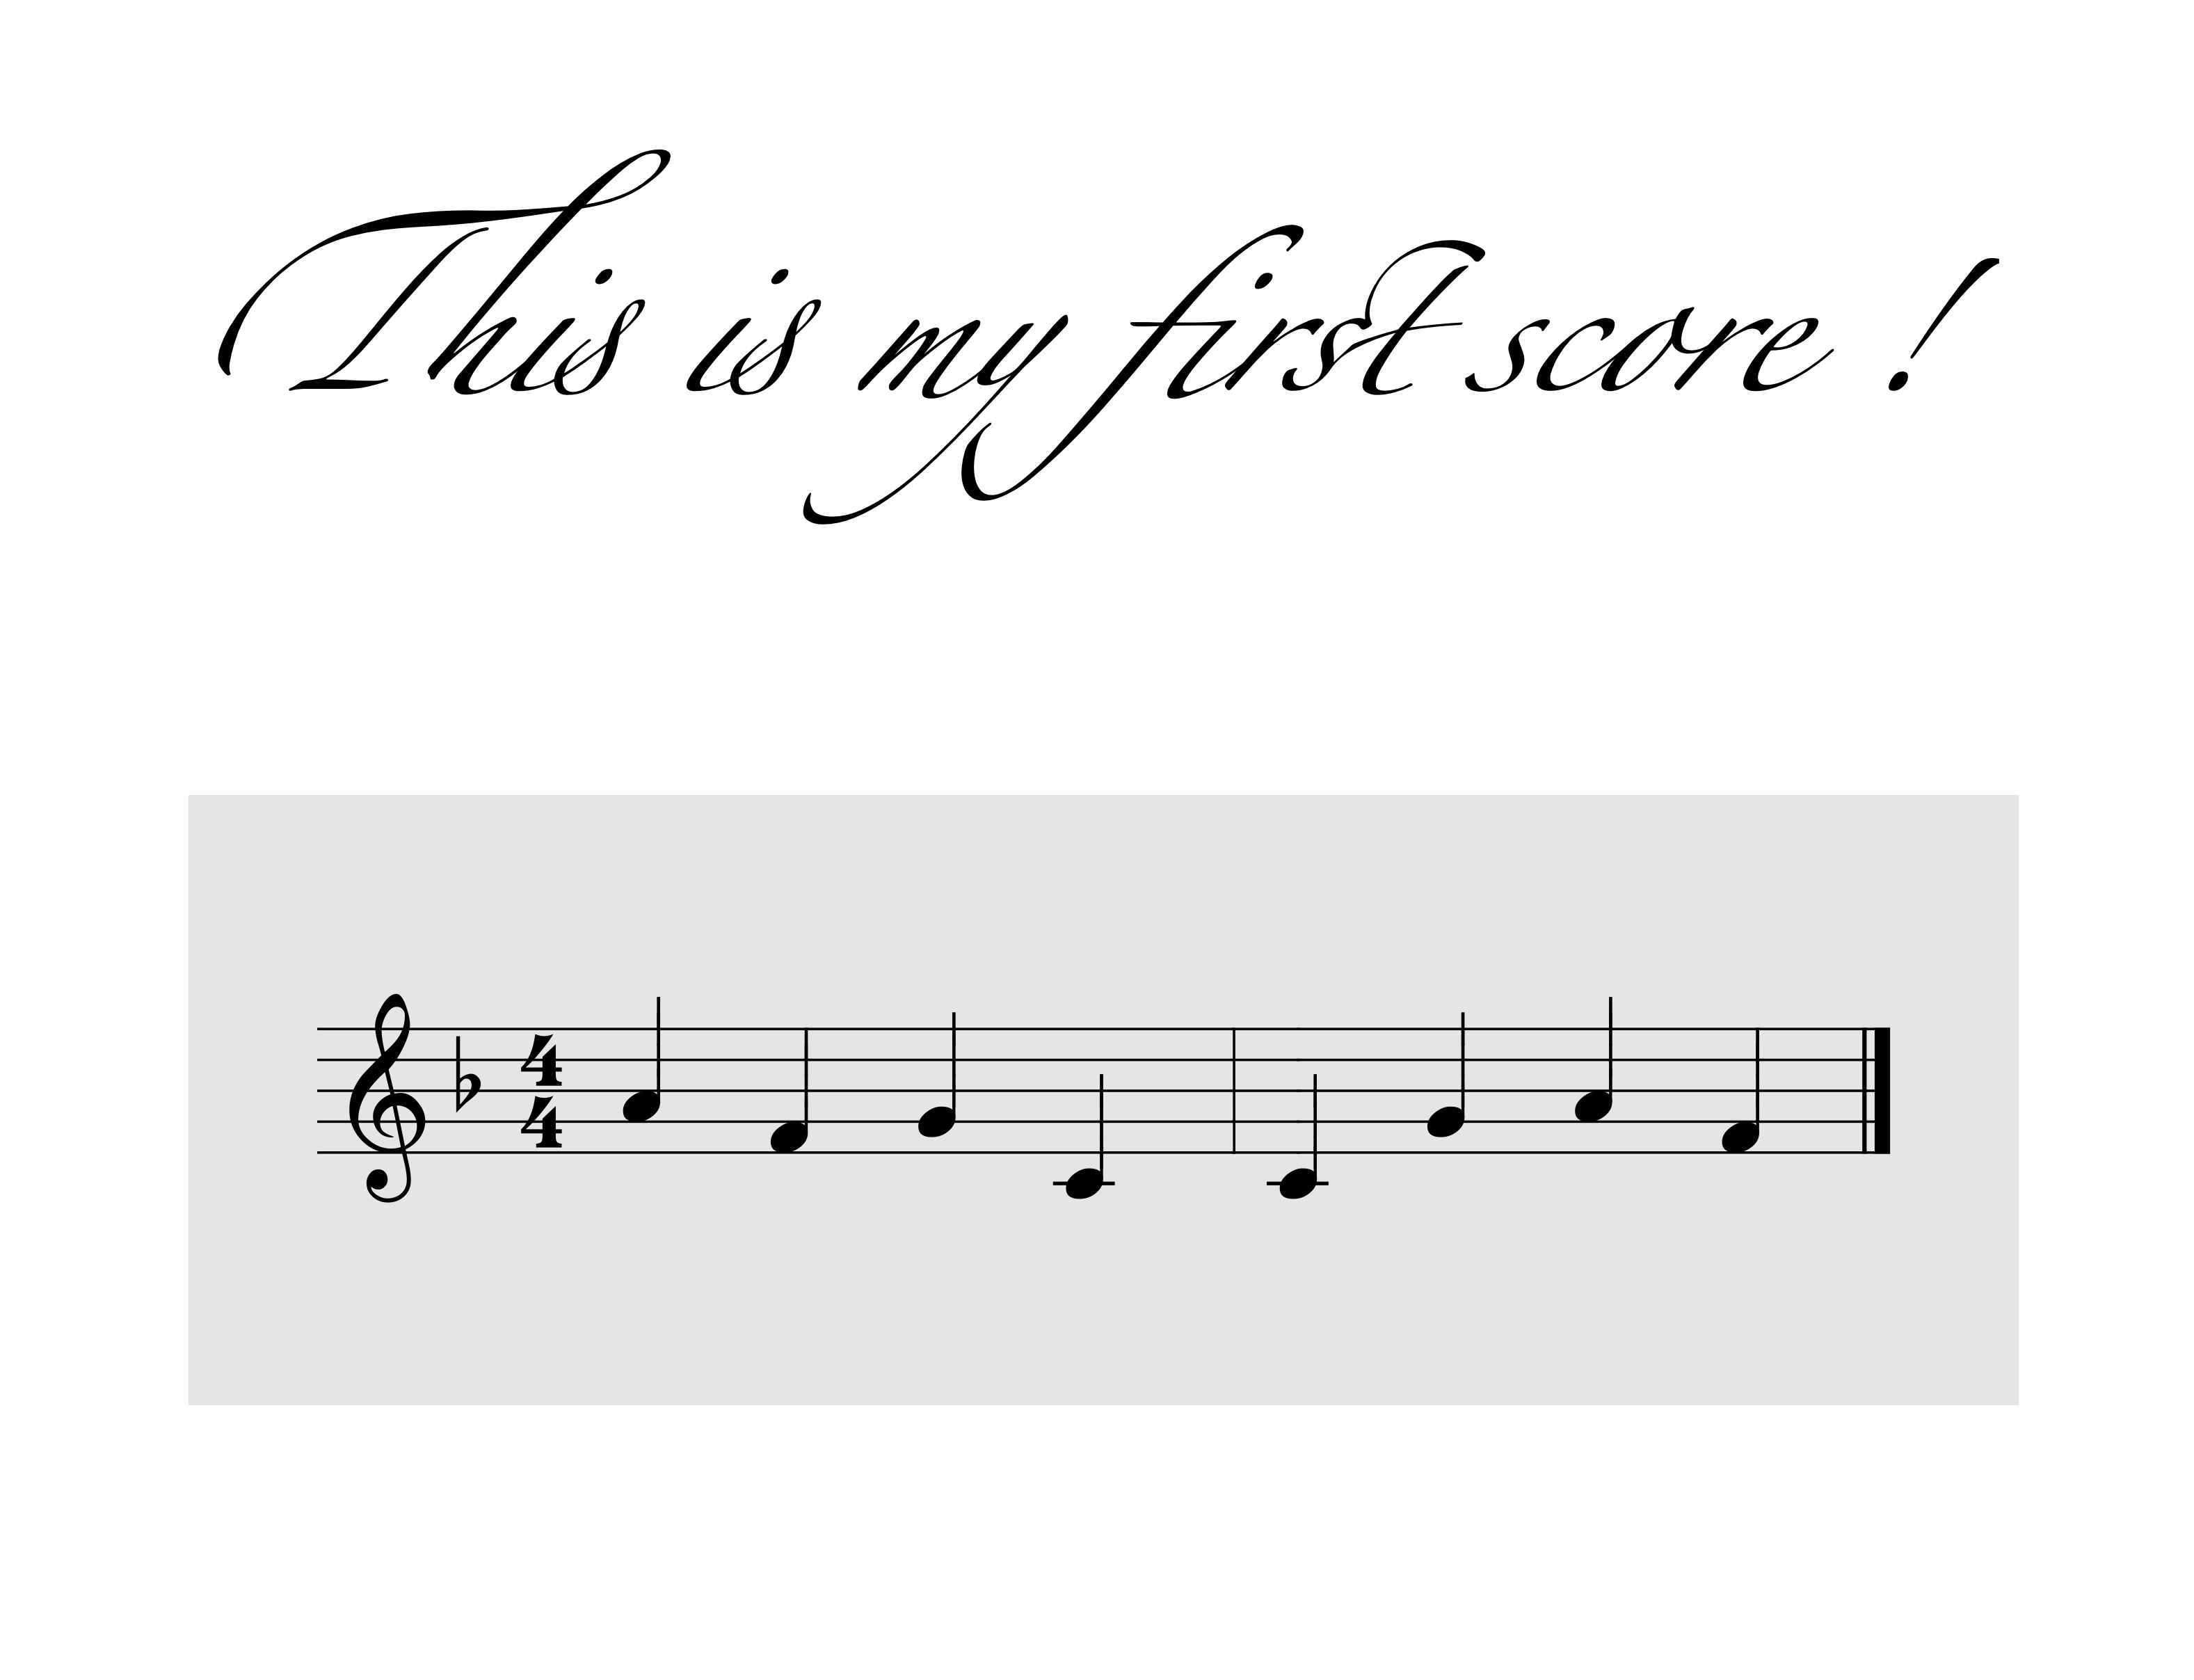
\includegraphics[width=0.7\columnwidth]{rsrc/inscore-exemple.png}
\caption{A simple score.}
\label{fig:score}
\end{figure}
In fact, the script above mixes two languages: the INScore language whose general form is `/address parameters...`, and the Guido language \cite{hoos98} which is used to specify the content of the \icode{score} element.

\section{INScore Web Architecture}\label{sec:arch}

INScore is based on a Model View Controller [MVC] architecture: the Model is an abstract description of the music score, it includes all the properties of the elements which are organised in a tree, in a strictly similar way to their OSC address. The View is a graphical representation of the Model.
The controller takes input messages, decodes them to modify the Model and when necessary, activates the refresh of the View at regular time intervals (every 10ms by default).
This architecture was used to differentiate the method of handling the Model and the View in the implementation for the Web.

\subsection{INScore Model as a WebAssembly library}

Mozilla developers have started in 2011 the Emscripten compiler project \cite{10.1145/2048147.2048224}, based on LLVM technology. From C/C++ sources, it allows to generate a statically compilable and garbage-collection free typed subset of JavaScript named asm.js. This first approach has successfully demonstrating that near native code performance could be achie-ved on the Web. It has been followed by WebAssembly\footnote{WebAssembly \url{https://webassembly.org/}} [WASM], a new efficient low-level programming language for in-browser client-side scripting, faster than the asm.js approach.

The existing INScore Model, developed in C++, was compiled with Emscripten to produce a WASM library. 
As a result, the native and the Web versions share the main of the code, which greatly minimises the maintenance of both platforms.

\subsection{INScore View as DOM based Javascript library}

INScore View has been developed using Typescript\footnote{Typescript \url{https://www.typescriptlang.org/}}, a language which builds on JavaScript, by adding static type definitions, allowing the TypeScript compiler to validate that your code is working correctly. It is compiled as a Javascript library.

The View implementation is entirely based on the Document Object Model [DOM] as defined by the W3C\footnote{DOM \href{https://www.w3.org/TR/2000/WD-DOM-Level-1-20000929/DOM.pdf}{Specification}}. It creates HTML elements on the fly and makes an extensive use of SVG. Most of the score objects properties are translated into style attributes (as defined by CSS).



\subsection{INScore Controller}

The controller lies in both the WASM and Javascript libraries as shown in figure \ref{fig:ctrl}. Actually, the only input of the INScore engine are text messages (unlike the native version which also accepts OSC messages). These messages can result from user actions or come from the network (see section \ref{sec:comm}). They are first parsed and then passed on to the objects of the Model.
\begin{figure}[H]
\centering
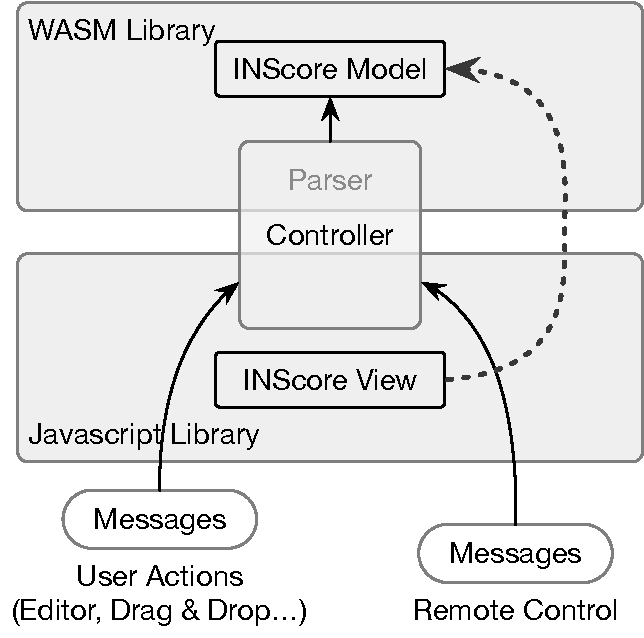
\includegraphics[width=0.7\columnwidth]{rsrc/controller.pdf}
\caption{INScore Controller design}
\label{fig:ctrl}
\end{figure}


%=========================================================
\section{Signal Processing extension}\label{sec:faust}

INScore Web can optionally embed the Faust compiler to provide signal processing objects within the score. 
Faust \cite{orlarey:hal-02159014} is a functional, synchronous, domain specific programming language working at the sample level, designed for real time audio signal processing and synthesis. Faust programs can be efficiently compiled to a variety of target programming languages, from C++ to WebAssembly. 

The Faust compiler is available as a WASM library \cite{letz:hal-02158925}. It is available as a NPM package\footnote{\href{https://www.npmjs.com/package/@grame/libfaust}{Faust NPM package}}, which includes also a Javascript library providing a high level API to transform DSP code into a Web AudioNode\footnote{\href{https://developer.mozilla.org/en-US/docs/Web/API/Web_Audio_API}{The Web Audio API}}.

The type of a Faust object is \icode{faust} and its \icode{set} method (figure \ref{fig:fset}) takes DSP code as argument. It is graphically represented by a browsable block diagram. Faust audio nodes can be instantiated as monophonic or polyphonic nodes, thus the \icode{set} method takes an optional number of voices as illustrated below. When present (and even if equal to 1), a polyphonic Faust audio node is created. 
\begin{figure}[h]
\centering
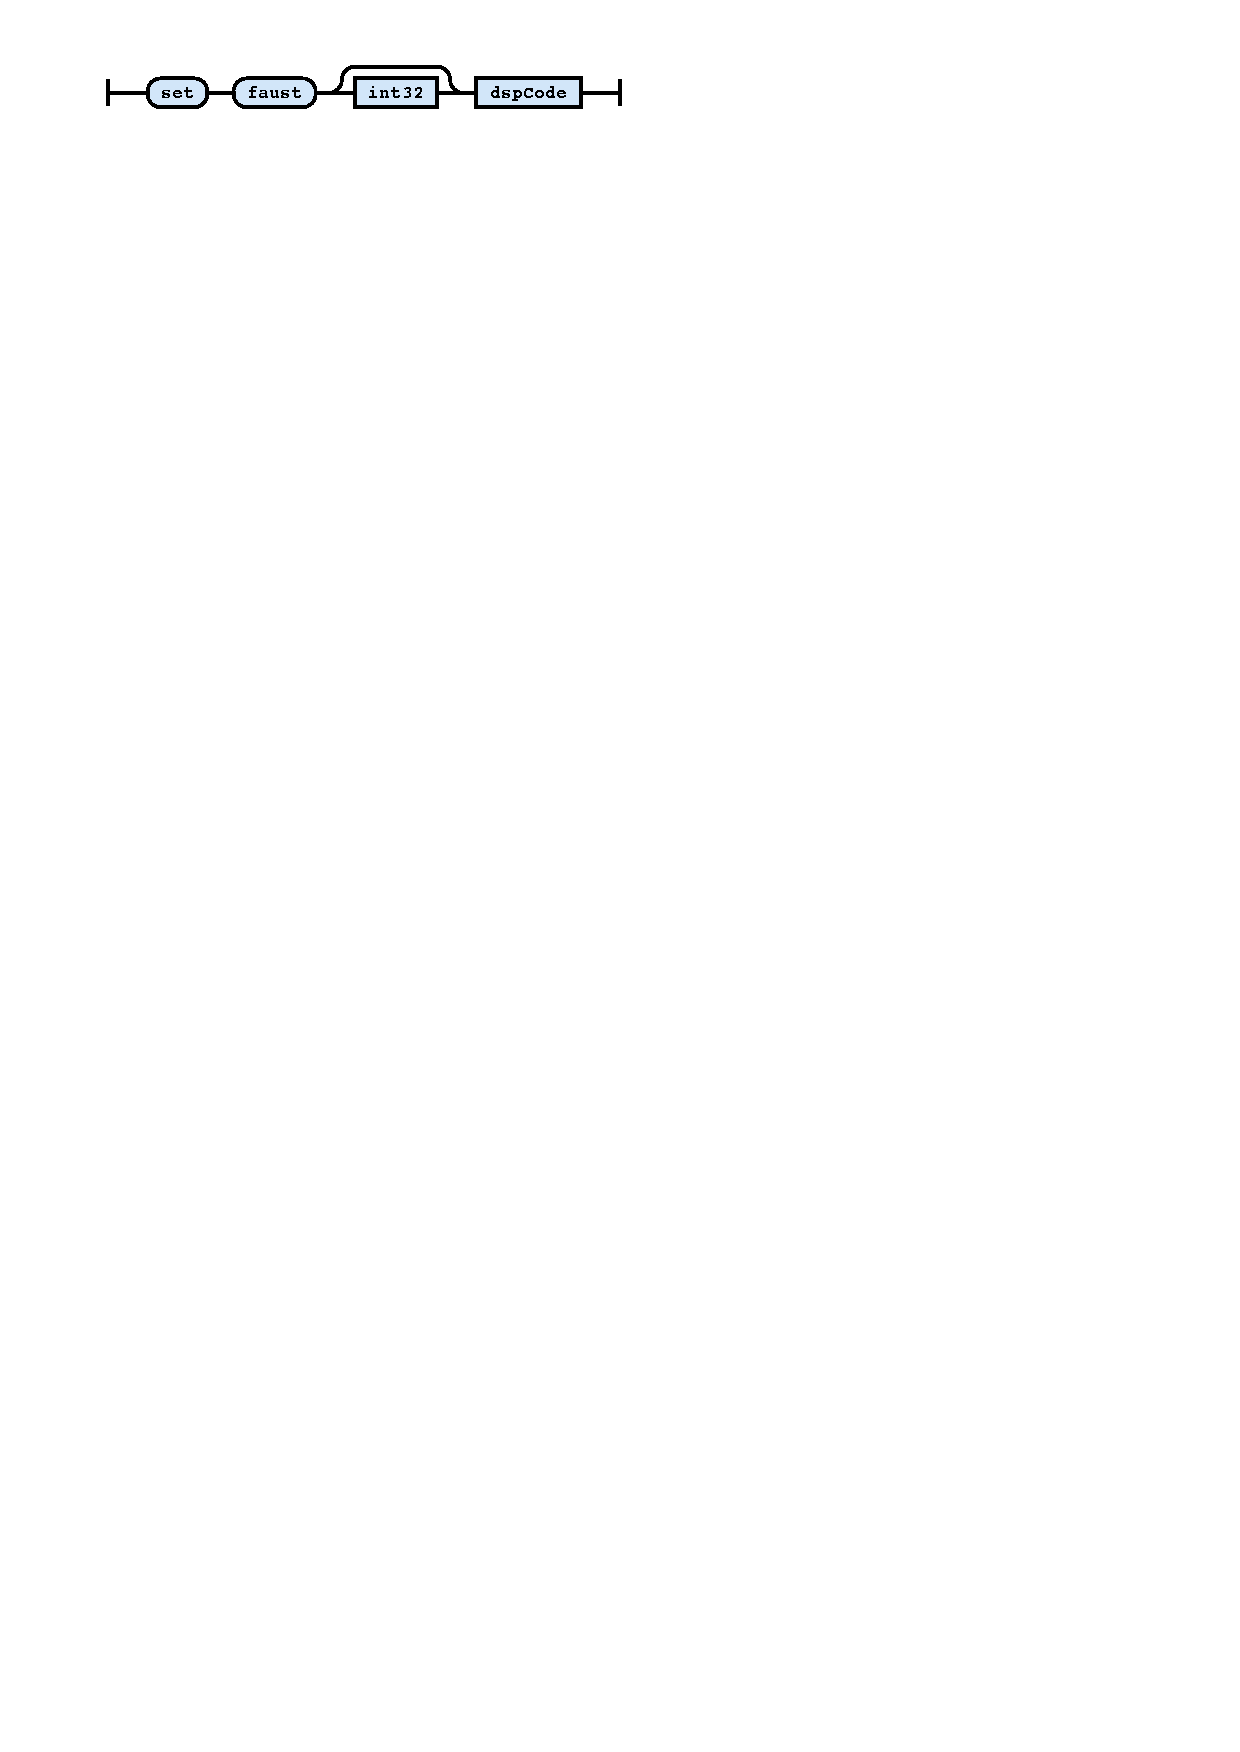
\includegraphics[width=0.9\columnwidth]{rsrc/faust1.pdf}
\caption{\icode{set} method of Faust objects.}
\label{fig:fset}
\end{figure}

The following code creates a monophonic object named \icode{karplus} using the Faust physical modeling library, that is a ready-to-use, MIDI-enabled Karplus-Strong string with built-in UI.
\code{/ITL/scene/karplus set faust \\
\hspace*{10mm} 'import("stdfaust.lib"); \\
\hspace*{11mm} process = pm.ks\_ui\_MIDI';}


\subsection{Faust objects methods}

Faust objects carry all the properties common to INScore objects, including their temporal dimension. 
Their specific methods are the following:
\begin{itemize}
\item[-] \icode{play}: start or stop the sound processing. Takes a boolean value ([01]) as argument.
\end{itemize}

The next methods are only supported by polyphonic objects:
\begin{itemize}
\ispace
\item[-] \icode{keyOn}, \icode{keyOff}: similar to MIDI key on/off messages. Take a MIDI channel, a pitch and a velocity as arguments.
\item[-] \icode{allNotesOff}: similar to MIDI all notes off message. 
\end{itemize}

Faust objects support also specific query (\icode{get}) methods, corresponding to read-only properties:
\begin{itemize}
\ispace
\item[-] \icode{in}, \icode{out}: gives the number of input and output signals of the Faust object.
\item[-] \icode{paths}: gives the interface to the Faust object UI (as defined by the DSP code).
\end{itemize}

Paths returned by the \icode{path} query are used internally to dynamically generate the address space of the Faust object (see section \ref{faustadrspace}), providing control over the Faust node parameters.

\subsection{Faust objects address space}\label{faustadrspace}

Faust provides user interface primitives that allow for an abstract description of a user interface within the Faust code. This description is independent from any GUI toolkits/frameworks and it's the responsibility of \emph{architecture files} \cite{Fober:11b} to instantiate this abstract description. In INScore, this abstract description is instantiated in the address space of the Faust object.
Let's consider the following query addressed to the \icode{karplus} object as defined by the example in section \ref{sec:faust}.

\code{/ITL/scene/karplus get paths;}

The INScore engine returns a list of UI elements as follows:
\code{/karplus/params/freq hslider freq 440.0 50.0 1000.0 0.01;\\
/karplus/params/bend hslider bend 0.0 -2.0 2.0 0.01;\\
/karplus/params/damping hslider damping 0.01 0.0 1.0 0.01;\\
etc.}
where the general form of an element is a sequence of
\begin{description}
\ispace
\item[] \icode{address}: the address of a Faust audio node parameter.
\item[] \icode{type}: the type of the UI element (ignored by INScore).
\item[] \icode{name}: the name of the UI element (ignored by INScore).
\item[] \icode{default}: the default value of the parameter.
\item[] \icode{min}: the minimum value of the parameter.
\item[] \icode{max}: the maximum value of the parameter.
\item[] \icode{step}: the step of values (ignored by INScore).
\end{description}

The \icode{address} field is used to expand the address space of the Faust object so that for the object \\
\icode{/ITL/scene/karplus}\\
 the addresses\\
\icode{/ITL/scene/karplus/karplus/params/freq} \\
\icode{/ITL/scene/karplus/karplus/params/bend} \\
etc. \\
become valid addresses taking a float value as argument, that is passed to the Faust audio node to set the corresponding parameter value. 


\section{Web communication}\label{sec:comm}

\subsection{Server Side}\label{sec:server}
INScore provides a \emph{fowarding} mechanism \cite{Fober:15b} that can be used to distribute scores over a local network.
The general form of the \icode{forward} message is illustrated in figure \ref{fig:forward}. It can be addressed to the application or to the scene level. The destination host is specified similarly to an url, by IP number or by host name, followed by a port number.
A filtering mechanism is also provided to select the messages to be forwarded.
\begin{figure}[h]
\centering
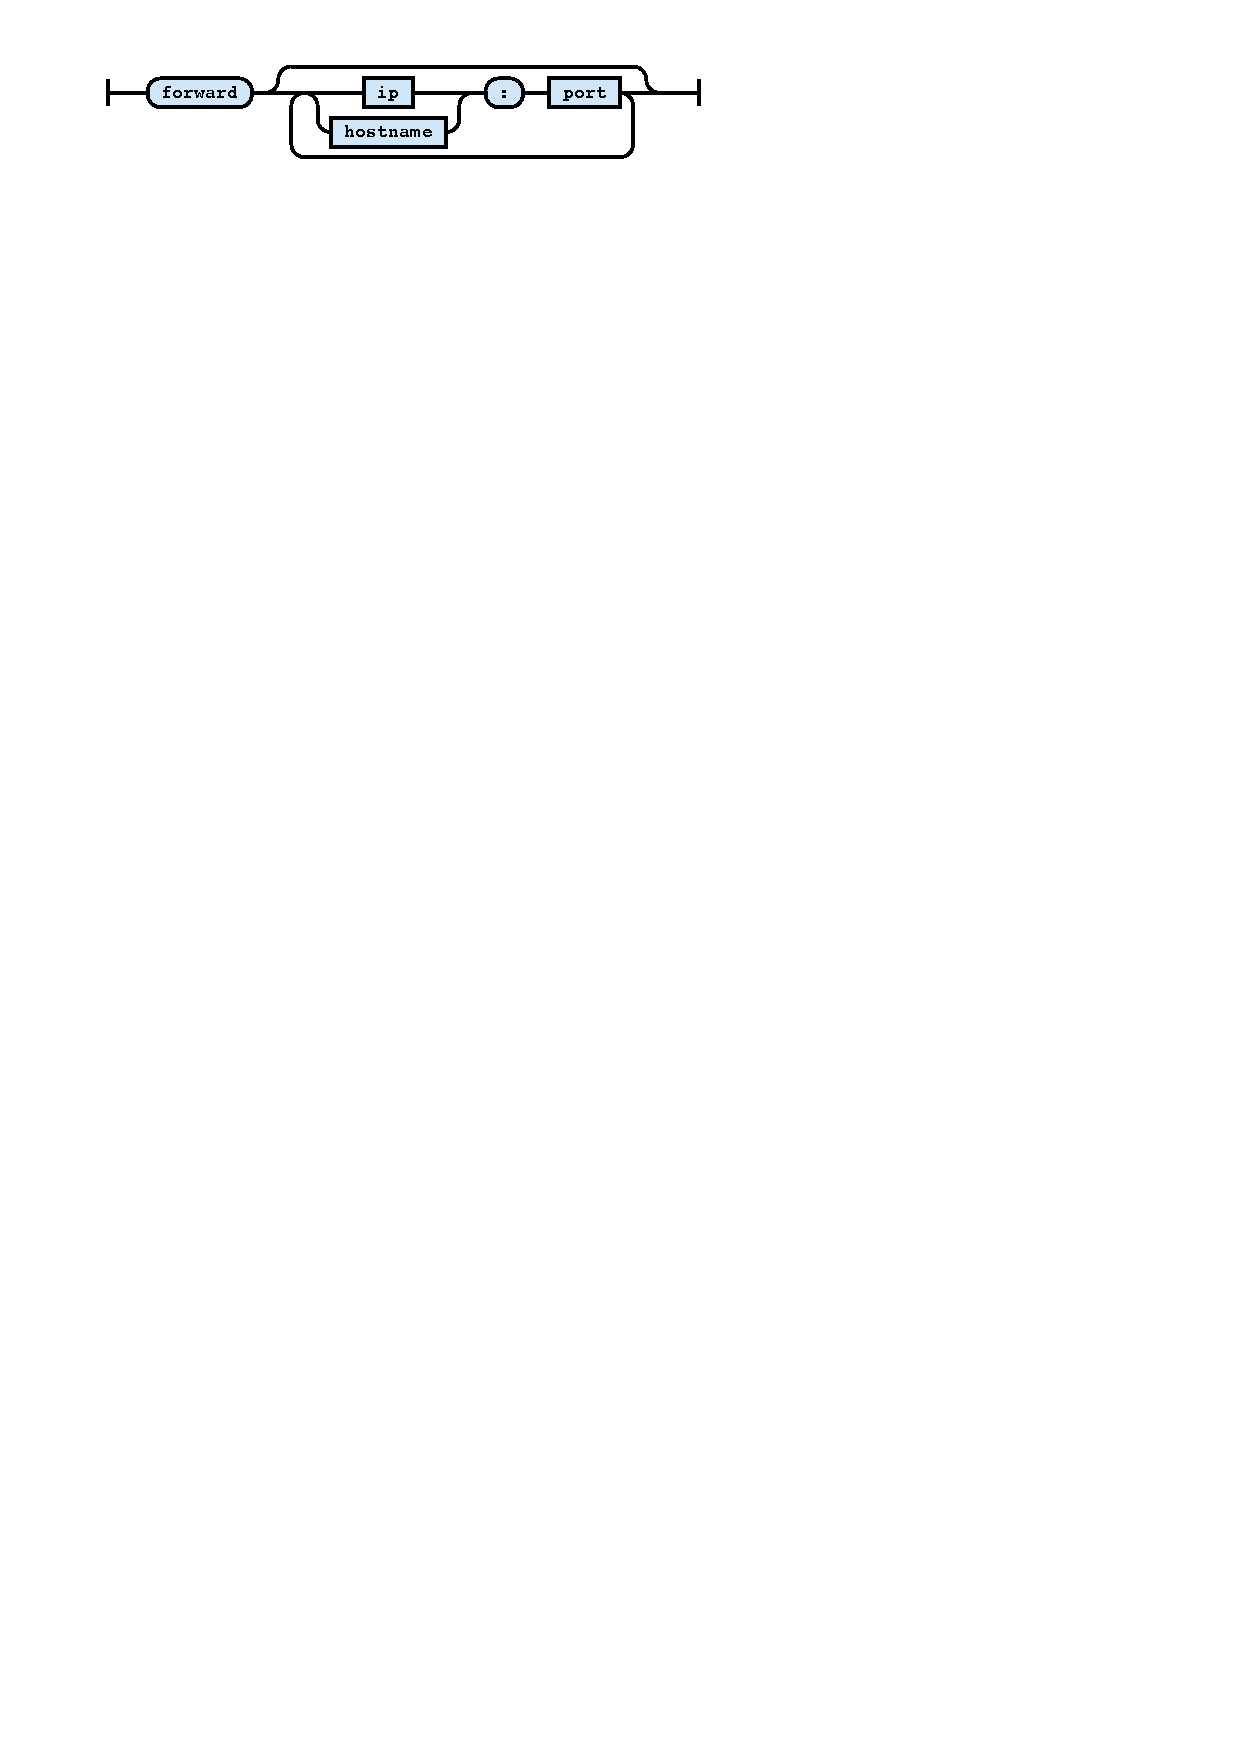
\includegraphics[width=0.7\columnwidth]{rsrc/faust3.pdf}
\caption{The \icode{forward} message.}
\label{fig:forward}
\end{figure}
This mechanism was basically design to transmit OSC message on UPD sockets.
It has been extended for the native INScore application, to support different protocols, namely Websockets and HTTP. The new form of the \icode{forward} message is illustrated in figure \ref{fig:newforward}.
\begin{figure}[h]
\centering
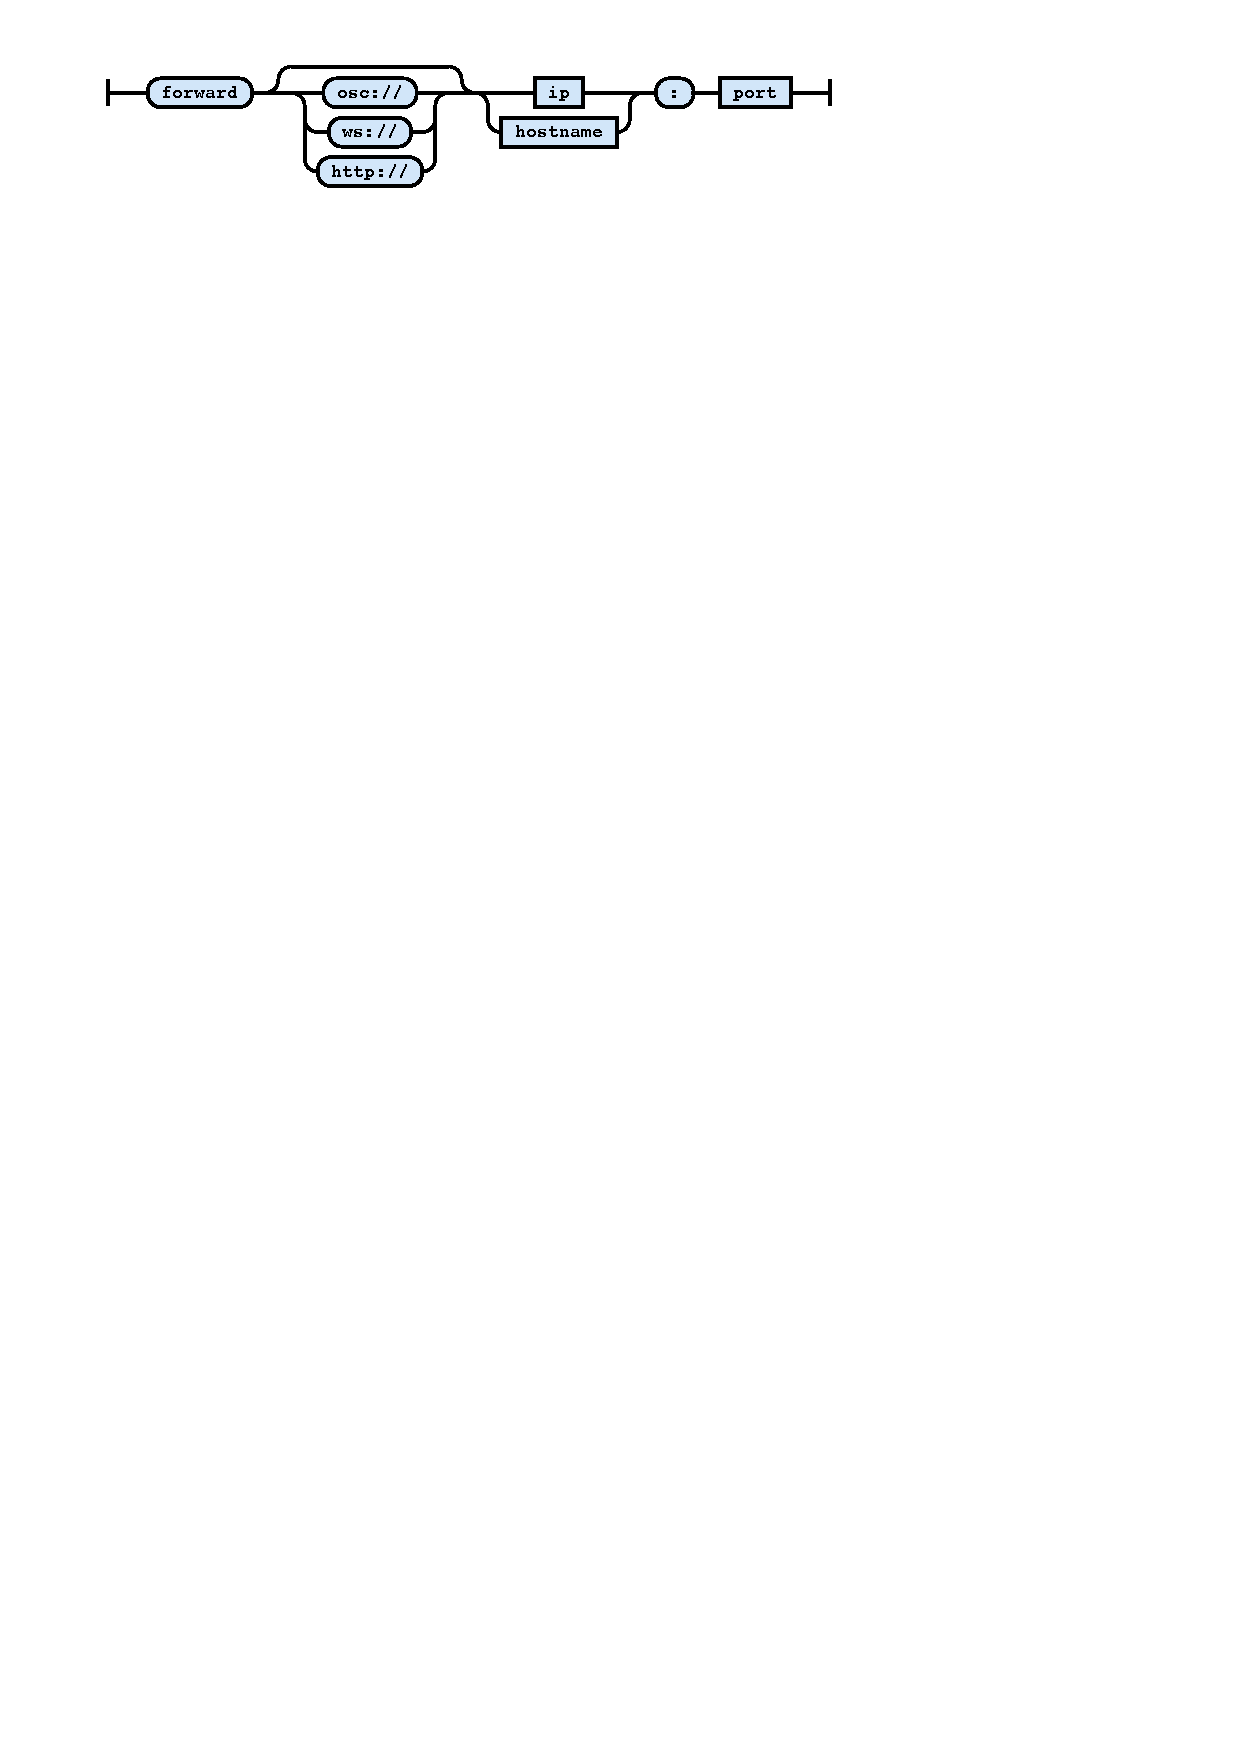
\includegraphics[width=0.98\columnwidth]{rsrc/faust4.pdf}
\caption{The new \icode{forward} message.}
\label{fig:newforward}
\end{figure}\\
\icode{osc://} \icode{ws://} and \icode{http://} refer respectively to the OSC protocol, to Websockets and to HTTP.
For compatibility reasons, the original form is preserved and implies the OSC protocol.

The OSC protocol runs over UDP and thus is connectionless, this is not the case for Websockets and HTTP that run over TCP.
Currently and whether for Websockets or HTTP, the INScore server ignores the host name and accepts all incoming connections. This approach may be revised in the future to select authorized hosts.

\subsection{Client Side}\label{sec:client}
The OSC protocol is transparent on client side: INScore has been natively designed to communicate via OSC.
For Websockets and HTTP, an explicit connection must be initiated by the client. 
For this we have introduced the \icode{connect} message whose form is similar to the \icode{forward} message. (figure \ref{fig:connect})
\begin{figure}[h]
\centering
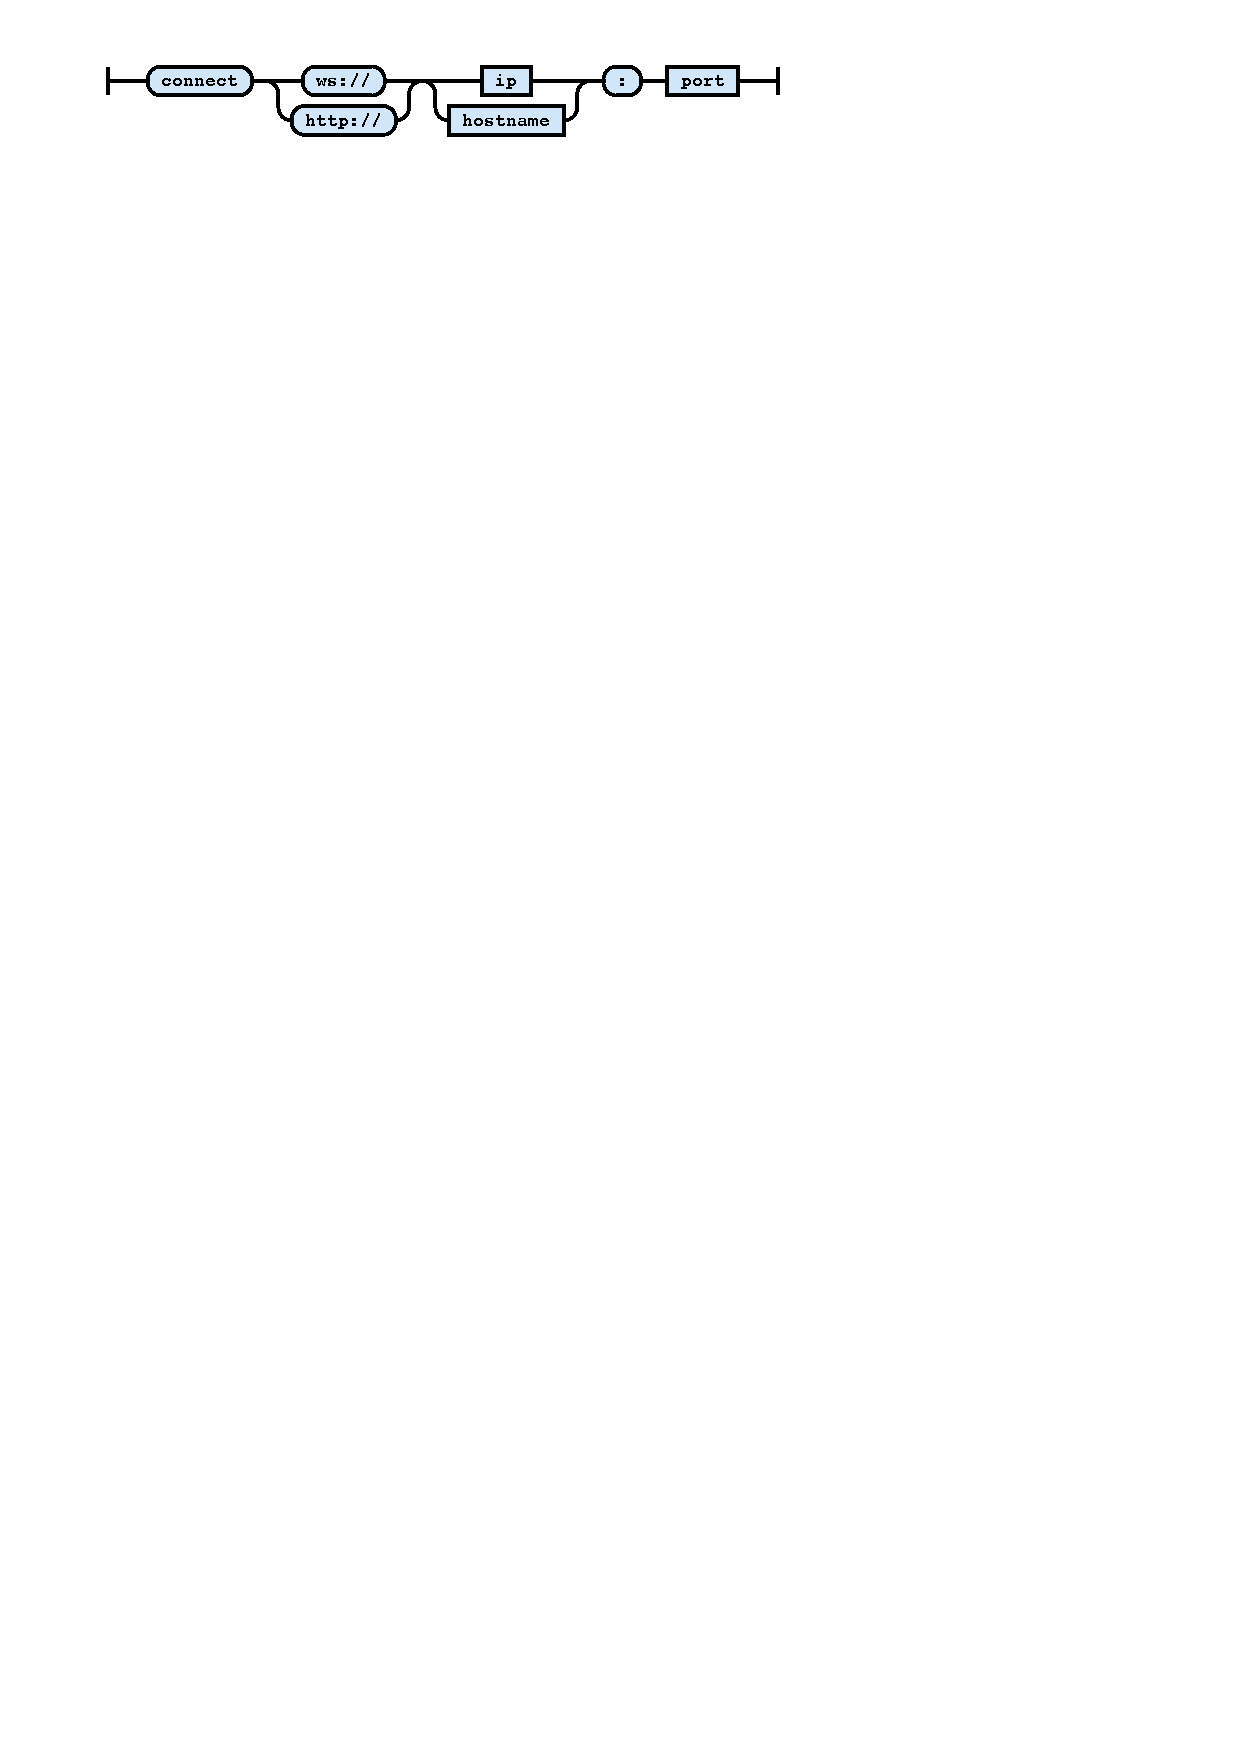
\includegraphics[width=0.98\columnwidth]{rsrc/faust5.pdf}
\caption{The \icode{connect} message.}
\label{fig:connect}
\end{figure}\\




%\begin{figure}[t]
%\centering
%\includegraphics[width=0.9\columnwidth]{figure}
%\caption{Figure captions should be placed below the figure, 
%exactly like this.
%\label{fig:example}}
%\end{figure}

%\begin{figure}[t]
%\figbox{
%\subfloat[][]{\includegraphics[width=60mm]{figure}\label{fig:subfigex_a}}\\
%\subfloat[][]{\includegraphics[width=80mm]{figure}\label{fig:subfigex_b}}
%}
%\caption{Here's an example using the subfig package.\label{fig:subfigex} }
%\end{figure}

\section{Conclusions}

%%%%%%%%%%%%%%%%%%%%%%%%%%%%%%%%%%%%%%%%%%%%%%%%%%%%%%%%%%%%%%%%%%%%%%%%%%%%%
%bibliography here
\balance
\bibliography{../interlude}

\end{document}
